\section{Disk emission in bumpy black holes spacetimes}\label{sec:emission}
The theory of thin accretion disks in the steady state was developed by \cite{1973A&A....24..337S} in the Newtonian case and generalised by \cite{1974ApJ...191..499P} to the general relativistic case. It is assumed that the disk lies in the equatorial plane with material moving in (approximately) circular geodesic orbits, with a small radial accretion velocity superposed on the circular motion. In addition, it is assumed that the disk is thin (i.e. at a radius $r$ the thickness $2h$ satisfies $h\ll r$; the disk height may depend on radius, $h=h(r)$, but for notational simplicity this dependence in suppressed here) and is in a steady state with a constant accretion rate $\dot{M}_{0}$. The disk extends from the innermost stable circular orbit (ISCO) of the spacetime to some finite outer radius (strictly, to be consistent with the steady state assumption, the disk must extend indefinitely; here the more conservative approach of leaving the outer radius as a free parameter is taken). When the accreting material reaches the ISCO it plunges quickly into the BH without radiating any further or interacting viscously with the material at larger radii. The fact that the material plunges quickly after crossing the ISCO provides the physical motivation for imposing a zero torque boundary condition at the inner edge of the disk. This allows the differential equation governing the radial dependence of the flux to be integrated; see Eq.\ \ref{eq:radialfluxmain}. 

The model described above is often referred to as the standard relativistic model of accretion disks, and has been extensively studied for the Kerr geometry. Here it is necessary to retain sufficient generality to perform the calculations for any of the bumpy black holes described in Sec.\ \ref{sec:spacetimes}. Since the disk is thin and assumed to lie in the equatorial plane we may switch from using Boyer-Lidquist polar-like coordinates to cylindrical-like coordinates. The metric near the equatorial plane is given by
\begin{equation}\label{eq:metriccylindrical} \textrm{d}s^{2} = g_{tt}\textrm{d}t^{2}+2g_{t\phi}\textrm{d}t\textrm{d}\phi +g_{rr}\textrm{d}r^{2} + g_{\phi\phi}\textrm{d}\phi ^{2} + g_{zz} \textrm{d}z^{2}\, , \end{equation}
where the metric components depend only on $r$; corrections that depend on $z$ enter at second order and are neglected because the disc is assumed to be thin. By a rescaling of the $z$ coordinate the metric component $g_{zz}$ may be set to unity without any loss of generality.

The metric in Eqs.\ \ref{eq:generalmetric} and \ref{eq:metriccylindrical} does not depend on the timelike or azimuthal coordinates, so the corresponding covariant components of the four-momentum are conserved, $p_{t}=-E$ and $p_{\phi}=L$. Using the metric to raise the indices on these momentum components gives the first two geodesic equations in first order form, where a tilde denotes an orbital quantity per unit mass of the test particle,
\begin{eqnarray}\label{eq:timegeo} 
\frac{\textrm{d}t}{\textrm{d}\tau} 	=\frac{\tilde{E}g_{\phi \phi}+\tilde{L}g_{t \phi}}{g_{t \phi}^{2}-g_{tt}g_{\phi \phi}}\, , \nonumber \\ 
\frac{\textrm{d}\phi}{\textrm{d}\tau} 	=-\frac{\tilde{E}g_{t\phi}+\tilde{L}g_{tt}}{g_{t \phi}^{2}-g_{tt}g_{\phi \phi}}\, ,
\end{eqnarray}
where $\tau$ is the proper time along the worldline of the orbiting test particle.

Because the material in the disk is orbiting in the equatorial plane the vertical component of it's four-velocity vanishes, $\textrm{d}z/\textrm{d}\tau=0$. Therefore, the third and final geodesic equation may be conveniently obtained from the normalisation condition of the four velocity;
\begin{equation}
\label{eq:norm4velocity}g_{\mu\nu}\frac{\textrm{d}x^{\mu}}{\textrm{d}\tau}\frac{\textrm{d}x^{\nu}}{\textrm{d}\tau}\equiv g_{\mu\nu}u^{\mu}u^{\nu}=-1 \, , 
\end{equation}
\begin{equation}
\label{eq:radialgeo}\Rightarrow \left(\frac{\textrm{d}r}{\textrm{d}\tau}\right)^{2} = \frac{V_{\textrm{eff}}(r)}{g_{rr}} \, , 
\end{equation}
where,
\begin{equation} V_{\textrm{eff}}(r)= \frac{\tilde{E}^{2}g_{\phi \phi}+2\tilde{L}\tilde{E}g_{t\phi}+\tilde{L}^{2}g_{tt}}{g_{t\phi}^{2}-g_{tt}g_{\phi\phi}}-1 \, . \end{equation} 
From Eq.\ \ref{eq:radialgeo} it can be seen that the conditions for stable circular orbits are $V_{\textrm{eff}}(r)\nobreak=\nobreak V_{\textrm{eff},r}(r)\nobreak=\nobreak0$, where a comma in the subscript denotes a partial derivative with respect to all subsequent indices. These two conditions yield expressions for the specific energy and angular momentum per unit mass of a particle on a circular, equatorial geodesic;
\begin{eqnarray} 
\tilde{E} = -\frac{g_{tt}+g_{t\phi}\Omega}{\sqrt{-\left( g_{tt}+2g_{t\phi}\Omega+g_{\phi\phi}\Omega^{2} \right)}} \label{eq:En} \\
\tilde{L} = \frac{g_{t\phi}+g_{\phi\phi}\Omega}{\sqrt{-\left( g_{tt}+2g_{t\phi}\Omega+g_{\phi\phi}\Omega^{2} \right)}}\; . \label{eq:Lz}
\end{eqnarray}
Combining Eqs.\ \ref{eq:timegeo} with Eqs.\ \ref{eq:En} and \ref{eq:Lz} gives an expression for the coordinate angular velocity of the particle,
\begin{equation}\label{eq:omega} \Omega = \frac{\textrm{d}\phi}{\textrm{d}t} = \frac{-g_{t\phi ,r}+\sqrt{ \left( g_{t\phi,r} \right)^{2} - g_{tt,r} g_{\phi\phi ,r} }}{g_{\phi \phi , r}} \; . \end{equation}

In the metrics of interest in this paper (i.e.\ the Kerr metric and small perturbations from it) there exists an ISCO. The radius of the ISCO may be found by solving $V_{\textrm{eff}, r r}(r)=0$ simultaneously with $V_{\textrm{eff}}(r)\nobreak=\nobreak V_{\textrm{eff},r}(r)\nobreak=\nobreak0$. This equation admits the following analytic solution in the Kerr case \citep{1972ApJ...178..347B};
\begin{eqnarray}\label{eq:KerrISCO}
&Z_{1}=1+\left(1-a^{2}\right)^{1/3}\left((1+a)^{1/3}+(1-a)^{1/3}\right) \; ,\nonumber\\
&Z_{2}=\left(3a^{2}+Z_{1}^{2}\right)^{1/2} \; , \nonumber\\
&r_{isco}= 3+Z_{2}-\left((3-Z_{1})(3+Z_{1}+2Z_{2})\right)^{1/2}\, .
\end{eqnarray}
For the general bumpy black holes discussed in Sec.\ \ref{sec:spacetimes} the radius for the ISCO must be found numerically. However, if the spacetime is characterised by a small deformation from Kerr, then the radius of the ISCO may be expanded perturbatively in the bump parameter, $\epsilon$,
\begin{equation}\label{eq:iscoshift} r_{isco}=r^{\textrm{Kerr}}-\epsilon \frac{ \left.\frac{\textrm{d}V_{\textrm{eff},rr}(r,\epsilon)}{\textrm{d}\epsilon}\right|_{r=r^{\textrm{Kerr}}_{isco},\epsilon=0} }{\left.\frac{\textrm{d}V_{\textrm{eff},rr}(r,\epsilon)}{\textrm{d}r}\right|_{r=r^{\textrm{Kerr}}_{isco},\epsilon=0}} +{\cal{O}}\left(\epsilon^{2}\right)\; .\end{equation}
If the metric is characterised by more than one bump parameter, $\epsilon_{i}$, as is the case with the ${\cal{B}}_{N}$ spacetimes described in Sec.\ \ref{sec:spacetimes} then the following replacement should be made in Eq.\ \ref{eq:iscoshift},
\begin{eqnarray} &\epsilon\left.\frac{\textrm{d}V_{\textrm{eff},rr}(r,\epsilon)}{\textrm{d}\epsilon}\right|_{r=r_{isco}^{\textrm{Kerr}},\epsilon=0} \rightarrow\sum_{i}\epsilon_{i}\left.\frac{\textrm{d}V_{\textrm{eff},rr}(r,\epsilon_{i})}{\textrm{d}\epsilon_{i}}\right|_{r=r^{\textrm{Kerr}}_{isco},\epsilon_{i}=0} .\nonumber\\
&\end{eqnarray}

From Eq.\ \ref{eq:omega}, and the fact that the orbit is circular and equatorial, the four-velocity of a small fluid element of the disk orbiting the black hole is given by
\begin{equation}\label{eq:circorbfourvel} \left( \frac{\textrm{d}t}{\textrm{d}\tau} , \frac{\textrm{d}r}{\textrm{d}\tau} , \frac{\textrm{d}\phi}{\textrm{d}\tau} , \frac{\textrm{d}z}{\textrm{d}\tau} \right) = \left(u^{t} , u^{r} , u^{\phi} , u^{z} \right) = u^{t} \left( 1,0,\Omega , 0 \right) \, ,\end{equation}
where $u^{t}$ may be found from the normalisation condition on the four velocity in Eq.\ \ref{eq:norm4velocity},
\begin{equation}\label{eq:four:vel} u^{t} = \frac{1}{\sqrt{-\left( g_{tt}+2\Omega g_{t\phi} +\Omega^{2}g_{\phi\phi} \right)}} \; .\end{equation}

Viscous forces in the disk cause the orbiting material to dissipate energy and gradually move inwards to smaller radii. An expression for the radial dependence of the flux of energy from the disk was derived in \cite{1974ApJ...191..499P}; for completeness this derivation is reproduced in Appendix \ref{app:b}. The resulting expression for the radial dependence of the flux is,
\begin{equation}\label{eq:radialfluxmain} F(r)=\frac{-\dot{M}_{0}\Omega_{,r}}{4\pi \sqrt{-{\bf{g}}}\left( \tilde{E}-\Omega \tilde{L} \right)^{2}} \int_{r_{\textrm{isco}}}^{r}\left(\tilde{E}-\Omega \tilde{L}\right) \tilde{L}_{,r}\, \textrm{d}r \; ,\end{equation}
where $\dot{M}_{0}$ is the accretion rate and ${\bf{g}}$ is the metric determinant. Since the disk is in thermodynamic equilibrium, and not heating up or cooling down, this flux of energy is radiated away from the disk in the form of a thermal distribution of photons.

\subsection{Line emission}\label{subsec:line}
In addition to the flux of thermal radiation a higher energy power-law component of hard X-ray photons is also observed \citep{1994MNRAS.269L..55Z}. For supermassive black holes with cooler disks this component can in fact dominate over the thermal component. The hard X-ray power-law component is generally believed to be caused by inverse compton scattering of the thermal photons radiated from the disk by the hot surrounding corona. A certain fraction of the hard X-ray photons are radiated back towards the disk surface where, upon incidence, they produce fluorescent transition lines which may also be observed as a third component of the spectrum. One frequently observed line is that due to the Iron (Fe) K$\alpha$ transition, which in its rest frame has an energy of $6.38\,\textrm{keV}$. The combined effects of gravitational redshifting and Doppler boosting broaden this line in to the characteristic shapes shown in Fig.\ \ref{fig:KerrLine}.

\begin{figure*}[t]
 \centering
 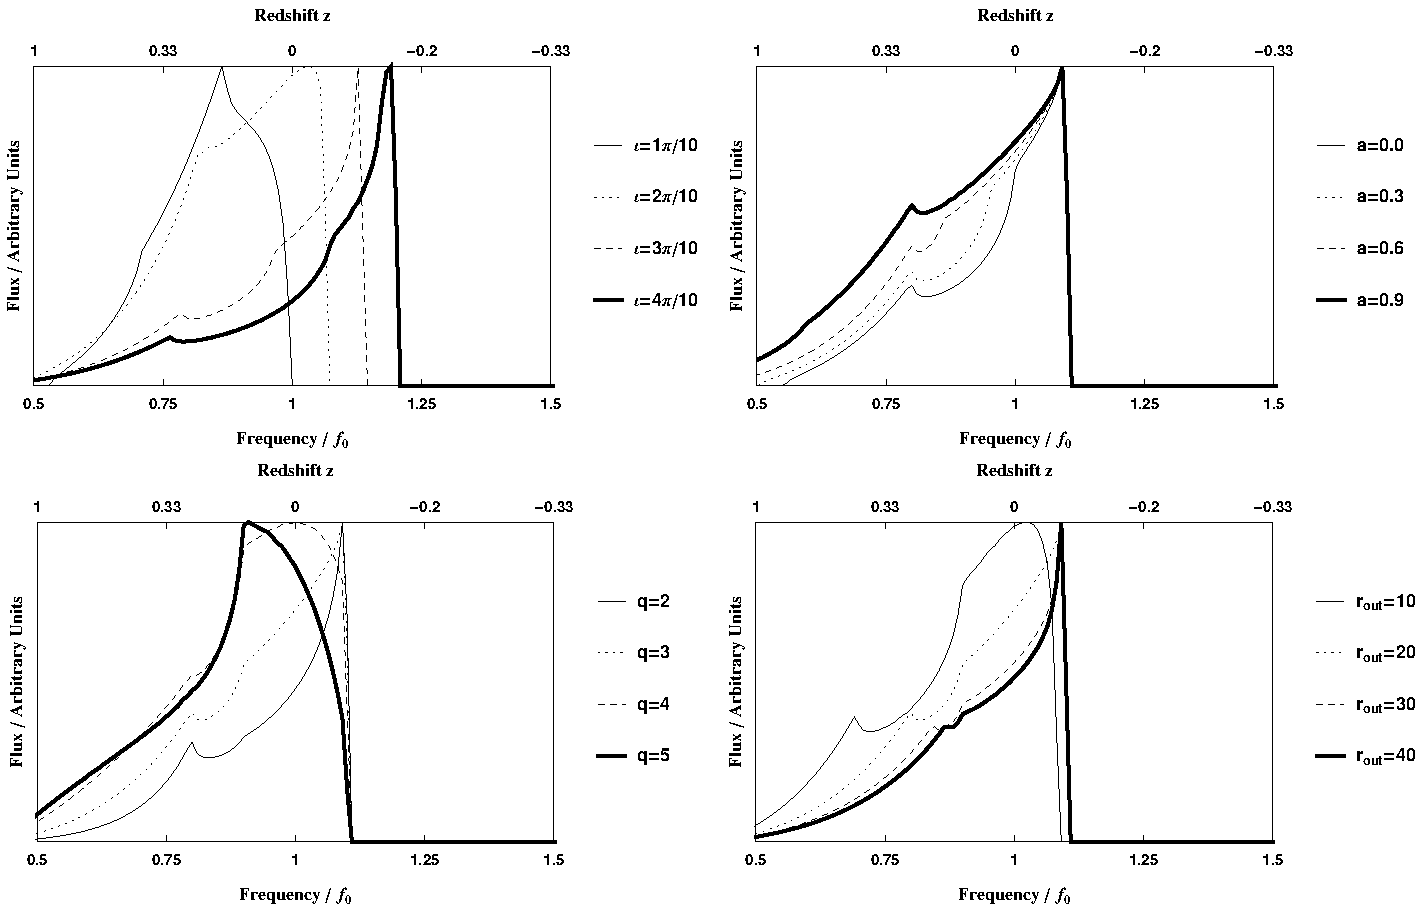
\includegraphics[trim=0cm 0cm 0cm 0cm, width=0.9\textwidth]{KerrLines.pdf}
 \caption{The dependence of the Kerr Iron line profile on various parameters. All spectra were normalised to the same peak flux. Unless otherwise stated in the figure all parameters were set to their fiducial values; $a=0.5$, $\iota=\pi/4$, $q=3$ and $r_{\textrm{out}}=30$.}
 \label{fig:KerrLine}
\end{figure*}

The observed line profile can be computed as follows. Let $\textrm{d}F_{0}(E_{0})$ be the infinitesimal element of flux at energy $E_{0}$ observed at infinity due to an infinitesimal element of the disk. If $I_{0}(E_{0})$ is the specific intensity (i.e.\ the energy per unit time, per unit area, per unit spectral energy (or frequency), per unit solid angle) in the observer's rest frame then
\begin{equation} \textrm{d}F_{0}(E_{0})=I_{0}(E_{0})d\Xi \; ,\end{equation}
where the element of the disk subtends solid angle element $d\Xi$. If the disk has a specific intensity $I_{e}(E_{e})$ in its own rest frame, given the invariance of $I/E ^{3}$ along the photon's worldline \citep{MTW}, it follows that
\begin{equation}\label{eq:fluxtemp1} \textrm{d}F_{0}(E_{0})=g^{3}I_{e}(E_{e})d\Xi \; , \end{equation}
where $g\equiv1/(1+z)\equiv E_{0}/E_{e}$ is the red-shift factor. For line emission the specific intensity may be approximated as a delta-function, $I_{e}(E_{e})=\epsilon (r_{e},\mu_{e})\delta (E_{e}-E_{int})$, where $E_{int}$ is the energy of the transition line in its rest frame, $\epsilon$ is the emissivity of the material, $r_{e}$ is the radius of the emitting fluid element and $\mu_{e}$ is the cosine of the angle of the emission with respect to the disk normal. Eq.\ \ref{eq:fluxtemp1} together with the delta-function expression for the line specific intensity gives
\begin{equation}\label{eq:fluxtemp2} \textrm{d}F_{0}(E_{0})=g^{4}\epsilon(r_{e},\mu_{e})\delta(E_{0}-gE_{\textrm{int}})d\Xi \; ; \end{equation}
the extra factor of $g$ in Eq.\ \ref{eq:fluxtemp1} compared to Eq.\ \ref{eq:fluxtemp2} comes from the change of argument in the delta-function. Now let $r_{e}$ and $\phi_{e}$ be the plane polar coordinates in the disk of the emitting point (where $\phi_{e}=0$ is along the line of nodes where the disk intersects the observers plane of the sky). In addition let $\alpha$ and $\beta$ be the cartesian coordinates in the observer's plane of the sky (where the $x$ axis appears to lie along the lines $\phi_{e}=0$ and $\phi_{e}=\pi$), and $r_{0}$ be the distance to the source. It follows that the solid angle element is given by $\textrm{d}\Xi = \textrm{d}\alpha \textrm{d}\beta / r_{0}^{2}$, and therefore integrating Eq.\ \ref{eq:fluxtemp2} gives
\begin{equation}\label{eq:fluxtemp3} F_{0}(E_{0})=\frac{1}{r_{0}^{2}} \iint\,\textrm{d}\,\alpha\, \textrm{d}\beta\; g^{4}\epsilon(r_{e},\mu_{e})\delta(E_{0}-gE_{\textrm{int}}) \; . \end{equation}
If light-bending is neglected then the polar coordinates of the emitting point in the disk ($r_{e}$ and $\phi_{e}$) may be related to the cartesian coordinates of the point in the observer's plane of the sky ($\alpha_{e}$ and $\beta_{e}$) via the transformation,
\begin{eqnarray}\label{eq:negligiblelightbenging} 
& \alpha_{e}=r_{e}\cos\phi_{e} \; , \;\; \beta_{e}=r_{e}\sin\phi_{e}\cos \iota\; , \nonumber \\
&\textrm{with Jacobian }\, \frac{\partial (\alpha,\beta)}{\partial (r_{e},\phi_{e})}=r_{e}\cos \iota \, ,\end{eqnarray}
where $\iota$ is the inclination from which the disk is viewed (i.e.\ the angle between the observer's line of sight and the spin axis of the BH). For further discussion of this assumption see Sec.\ \ref{subsec:lightbendingcalcs}. With this in hand we may change the integral in Eq.\ \ref{eq:fluxtemp3} from being over the observer's plane of the sky to being over the disk itself (Dropping the subscript $e$),
\begin{equation}\label{eq:fluxtemp4} F_{0}(E_{0})=\frac{\cos \iota}{r_{0}^{2}}\int_{0}^{2\pi}\int_{r_{isco}}^{r_{out}}r\textrm{d}r \textrm{d}\phi\, g^{4}\epsilon (r,\mu)\delta\left(E_{0}-gE_{int}\right)\, .\end{equation}

Hereafter the emissivity is taken to be a function of $r$ only (no $\mu_{e}$ dependence), and is parameterised as a power law, $\epsilon=r^{-q}$ where $q$ will be referred to as the emissivity index. We have now reduced the problem to finding the red-shift factor as a function of the position in the disk. The red-shift factor is defined by
\begin{equation} g \equiv \frac{E_{0}}{E_{e}} = \frac{p_{\mu}v^{\mu}\big|_{\textrm{observer}}}{p_{\mu}u^{\mu}\big|_{\textrm{emitter}}} \; ,\end{equation}
where $p_{\mu}$ is the four-momentum of the photon linking the emitter to the observer, $v^{\mu}$ is the four-velocity of the observer, and $u^{\mu}$ is the orbital four-velocity of the emitter (see Eq.\ \ref{eq:circorbfourvel}). Since the metric is independent of both the $t$ and $\phi$ coordinates, the corresponding components of the photon's four-momentum are conserved;
\begin{equation} \left[ p_{\mu} \right] = (p_{t},p_{r},p_{\theta},p_{\phi}) = (-E,p_{r},p_{\theta},\Lambda) \, .\end{equation}
If the observer is at infinity and is at rest with respect to the black hole the numerator of Eq.\ \ref{eq:redshiftfac} is simply given by ${p_{\mu}v^{\mu}\small|_{\textrm{observer}}=-E}$. Using the orbital four-velocity from Eq.\ \ref{eq:circorbfourvel} the denominator of Eq.\ \ref{eq:redshiftfac} is ${p_{\mu}u^{\mu}\small|_{\textrm{emitter}}=-Eu^{t}+\Omega u^{t} \Lambda}$, and hence the red-shift factor is given by
\begin{equation}\label{eq:redshiftfac} g=  \frac{1}{u^{t}(1-\Omega \lambda)} \; ,\end{equation}
where $\lambda = \Lambda /E$. Since $\lambda$ is conserved along the photon's worldline it may be evaluated at infinity where the indices on the photon four-momentum may be raised and lowered using the usual Minkowski metric. At large distance the ratio of the contravariant components of the photon's four-momentum gives the azimuthal impact parameter $\alpha$, defined in Eq.\ \ref{eq:negligiblelightbenging},
\begin{equation} \alpha = -\frac{r p^{\phi}}{p^{t}} \Big|_{r\rightarrow \infty} =-\frac{\lambda}{\sin\iota}\; .\end{equation}

\begin{figure}[h]
 \centering
 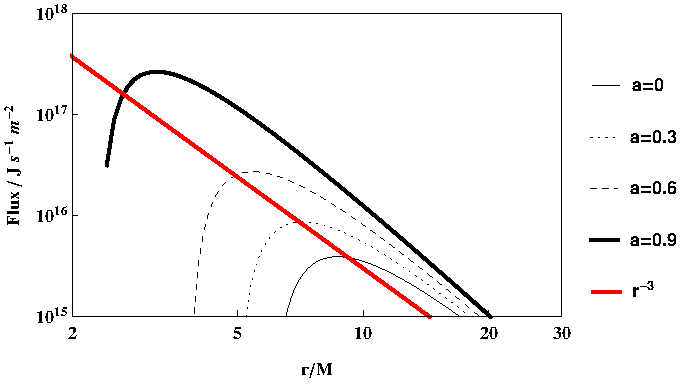
\includegraphics[trim=0cm 0cm 0cm 0cm, width=0.45\textwidth]{KerrFlux.pdf}
 \caption{The Flux as a function of radius, for various values of the spin parameter. Also shown is the power law, $(r/M)^{-3}$. All other parameters were set to their fiducial values, $\iota=\pi/4$, $M=\Msun$, $\dot{M}_{0}=10^{-12}\Msun/\textrm{yr}$ and $r_{\textrm{out}}=30$.}
 \label{fig:KerrFlux}
\end{figure}

If light-bending is neglected then the photon linking the emitting point in the disk to the observer at infinity travels on a straight line with impact parameter $\alpha = r\cos\phi $ (see Eq.\ \ref{eq:negligiblelightbenging}). Substituting these results into Eq.\ \ref{eq:redshiftfac} gives the red-shift;
\begin{equation} g\left(r,\phi \right)=\frac{\sqrt{-\left( g_{tt}+2\Omega g_{t\phi}+\Omega^{2}g_{\phi\phi} \right)}}{1+\Omega r \cos \phi \sin \iota} \, . \end{equation}
The flux integral in Eq.\ \ref{eq:fluxtemp4} may now be simply evaluated numerically. This was done initially for the unperturbed Kerr metric in order to reproduce known results (see, for example, \cite{1991MNRAS.250..629K,1991ApJ...376...90L}) and examine the dependence of the spectra on various parameters. The results of these calculations are shown in Fig.\ \ref{fig:KerrLine}. For all calculations in this paper, unless otherwise stated, the disk parameters were set to the following fiducial values; $a=0.5$, $\iota=\pi/4$, $q=3$ and $r_{\textrm{out}}=30$.

It can be seen from Fig.\ \ref{fig:KerrLine} that the profile is strongly sensitive to disk inclination. Qualitatively this is because the orbiting material is moving at relativistic speeds and for large inclinations material on one side of the disk is moving towards the observer while on the other side it is moving away. This produces both a blue and a red-shifted horn to the profile, the blue-shifted horn is always more intense due to the relativistic beaming effect which enhances the intensity of light emitted in the direction of travel (the headlight effect). 

\begin{figure*}[t]
 \centering
 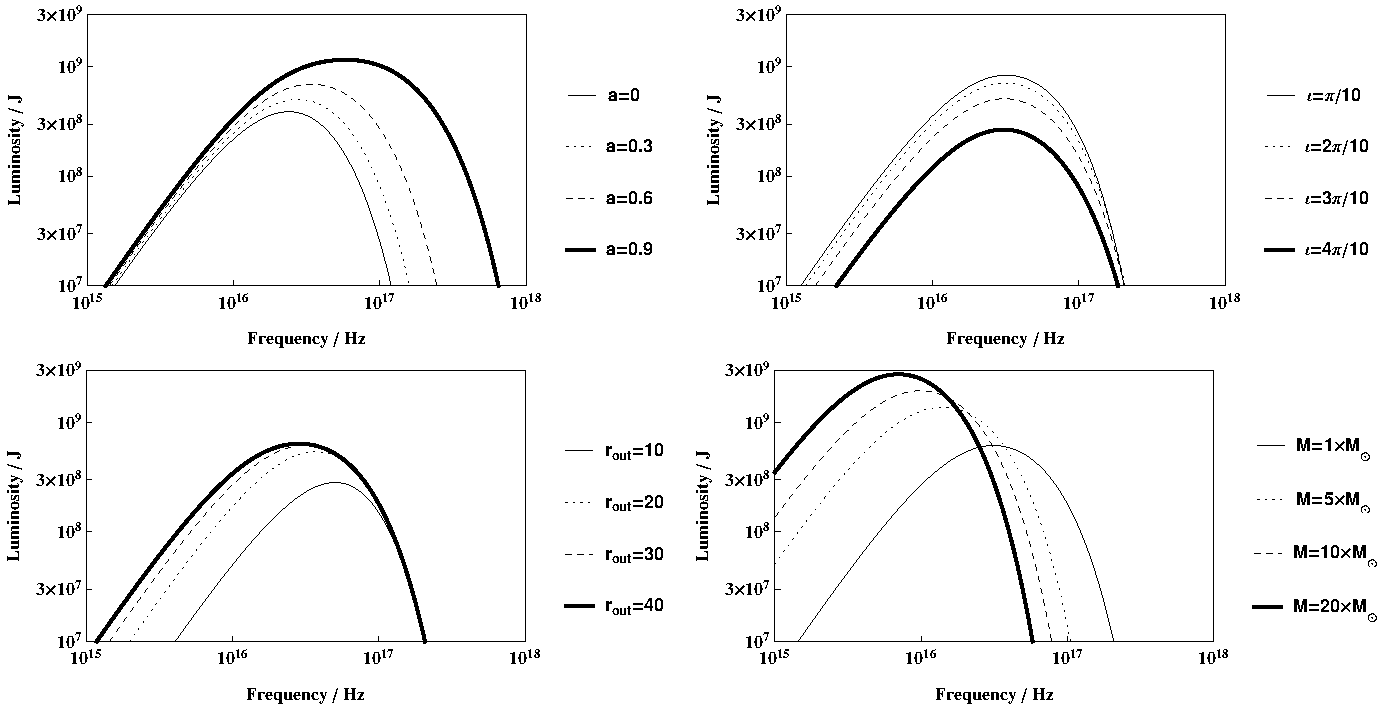
\includegraphics[trim=0cm 0cm 0cm 0cm, width=0.9\textwidth]{KerrTherm.pdf}
 \caption{The dependence of the Kerr black body spectrum on various parameters. Unless indicated otherwise all parameters were set to their fiducial values, $a=0.5$, $\iota=\pi/4$, $M=\Msun$, $\dot{M}_{0}=10^{-12}\Msun/\textrm{yr}$ and $r_{\textrm{out}}=30$.}
 \label{fig:KerrTherm}
\end{figure*}

The profile is also strongly sensitive to the radius of the inner edge of the disk, which in the Kerr case (under the modelling assumptions made here) is monotonically related to the spin parameter, $a$ (see Eq.\ \ref{eq:KerrISCO}). For higher spins (and smaller values of $r_{isco}$) it can be seen from Fig.\ \ref{fig:KerrLine} that the red-shifted wing of the line profile is much more prominent. Under the assumptions that the black hole is Kerr and the inner edge of the disk is located at the ISCO the line profile can be used as an accurate probe of the black hole spin, indeed such observations are among the best evidence for the existence of near maximally spinning black holes in some active galactic nuclei (see, for example, \cite{1996MNRAS.279..837I}). 

The line profile also depends strongly on $q$; this parameter must be fit for simultaneously with all other parameters. The fiducial value $q=3$ was chosen as this is approximately the form of the gravitational energy release per unit area of the disk (see Fig.\ \ref{fig:KerrFlux}). Likewise the value of $r_{out}$ must also be fit for, but this is less problematic because (at least for $r_{out}\gtrsim 20$) the profile only depends weakly $r_{out}$.


\subsection{Black-body spectra}\label{subsec:therm}
The line emission profiles calculated above encode how the gravitational and Doppler shifting (and lightbending if included) affect a single frequency source in the disk. If instead there is a broadband source the resulting spectrum may be obtained by convolving the spectrum in the source's rest frame with the line profile obtained in the preceding section. This method can be used to calculate the black body spectra by convolving with the Plank distribution of a black body; this approach is described by \cite{1975ApJ...202..788C}.

Here we take the alternative, and more physically motivated approach of directly integrating the flux over the disk to find the spectra. From Eq.\ \ref{eq:fluxtemp4} the radial flux (shown in Fig.\ \ref{fig:KerrFlux}) is known, and assuming that the radiation is that of a black body the Stefan-Boltzmann law gives the radial temperature distribution in the disk
\begin{equation} T(r)=\left( \frac{F(r)}{\sigma} \right)^{1/4} \; ,\end{equation}
where $\sigma$ is the Stefan-Boltzmann constant. Hence the thermal spectrum may be written as the following integral where the gravitational effects on the spectrum are included through the redshift factor,
\begin{equation}\label{eq:intforthermem}F_{0}(E_{0})=\frac{8\cos \iota}{\pi}\int_{r_{isco}}^{r_{out}}\int_{0}^{2\pi}r\textrm{d}\phi\,\textrm{d}r\;\frac{E_{0}^{3}}{g^{3}\left(e^{\frac{E_{0}}{gT}}-1\right)}\; .\end{equation}
As was the case for the line emission in Eq.\ \ref{eq:fluxtemp4}, the thermal spectrum in Eq.\ \ref{eq:intforthermem} is now in the form an integral over the disk in $r$ and $\phi$ coordinates; this was evaluated numerically. Several example thermal spectra are shown for the Kerr metric in Fig.\ \ref{fig:KerrTherm}.

The thermal spectra of the disk is the convolution between the line emission spectra and the Planck distribution. Since the Planck distribution contains no information about the gravitational field the thermal spectra in Fig.\ \ref{fig:KerrTherm} contain the same information about the black hole as the line spectra in Fig.\ \ref{fig:KerrLine}, only significantly smoothed out. Because of this smoothing it appears that the thermal spectra are less distinctive, and that therefore it would be harder to measure the parameters of the black hole using thermal emission than line emission. However, the thermal spectra may be observed across a much wider frequency range and at a larger signal-to-noise ratio. Therefore it is not obvious \emph{a priori} which method offers the best opportunity to constrain the metrics in Sec.\ \ref{sec:spacetimes}. In practice the most suitable technique depends upon the mass of the black hole; Iron line emission is typically most suitable for supermassive black hole whilst thermal emission is used for the hotter disks around stellar mass black holes. In rare instances both techniques may be used simultaneosuly, and they have been demonstrated to give consistent resuts \cite{2011MNRAS.416..941S}. Henceforth we consider only the Iron line emission, and we leave a detailed study of parameter estimation using thermal emission to future work. 

\subsection{The effect of lightbending}\label{subsec:lightbendingcalcs}
The formalism for calculating both the Iron line and thermal emission outlined in the preceding sections assumed that points in the image plane could be related to points in the disk by \emph{straight lines}, in the sense that the Boyer-Lindquist-like coordinates were treated as if they were spherical polar coordinates in flat space (these assumptions are summarised in Eq.\ \ref{eq:negligiblelightbenging}). As the light originates from the strong gravitational field the effects of lightbending (including frame dragging, if $a\neq 0$) may be significant. 

On the other hand it may be hoped that the effect of lightbending will vary slowly with changing system parameters, $\vec{\theta}$. If this is the case then while the inclusion of lightbending will have a significant impact on the observed profile it will have only a limited effect on our ability to measure the disk parameters, and hence on our ability to constrain deviations from the Kerr metric. In the language of the Fisher matrix calculations in Sec.\ \ref{sec:analysis}, even if the spectra depends strongly on whether or not lightbending is included if the derivatives of the spectra do not the the fisher matrix remains unchanged. In order to test the validity of this assumption a small number of calculations were performed including the effect of lightbending, and the results compared.

\begin{figure*}[t]
 \centering
 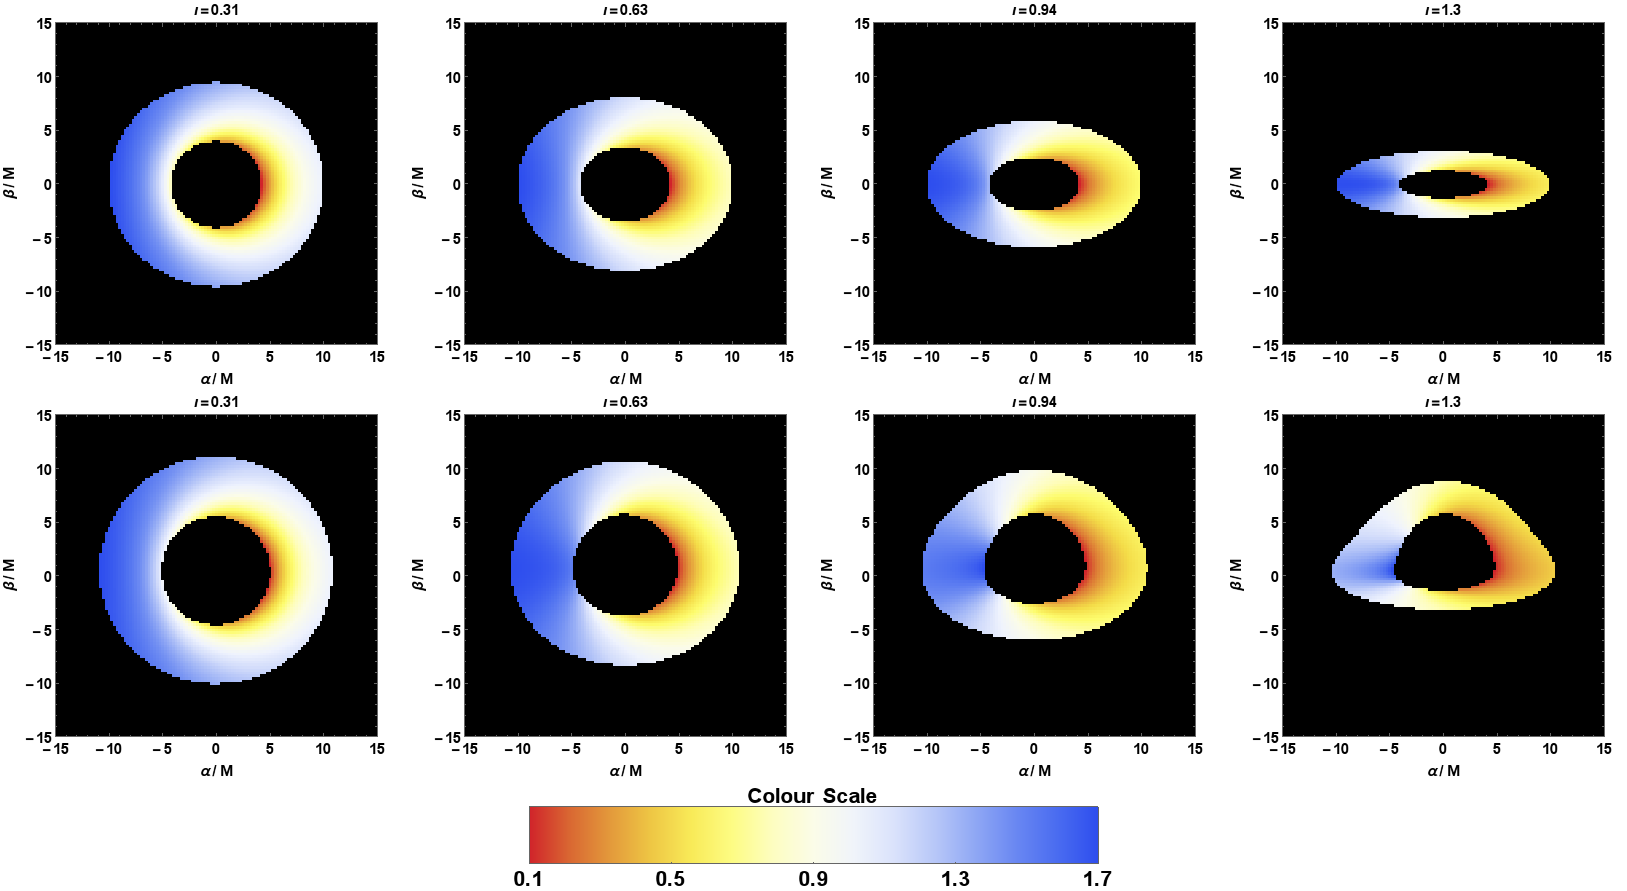
\includegraphics[trim=0cm 0cm 0cm 0cm, width=0.85\textwidth]{LightBendingDisk.png}
 \caption{A set of images showing the resolved appearance of an accretion disk around a Kerr black hole. The colour indicates the redshift of the light from that portion of the disk; the top row shows the disk with no lightbending and the bottom row shows the disk including lightbending. The inclination angle is varried between plot; from left to right it takes the values $\iota =\left\{\pi /10 , 2\pi /10 , 3\pi /10 , 4\pi /10 \right\}$. The spin parameter and outer radius of the disk were fixed to $a=0.5$ and $r_{out}=10$.}
 \label{fig:LightBendingDisk}
\end{figure*}

A method for ray-tracing photons from the image plane to the disk was outlined in \cite{2012ApJ...745....1P}. The method uses the fact that the spacetime is stationary and axisymmetric to write the $t$ and $\phi$ geodesic equations for the photon in first order form, but integrates the $r$ and $\theta$ geodesic equations in second order form. This is ideal for our present purpose as the method does not require the existence of a Carter-like constant, which does not exist in all the metrics discussed in Sec.\ \ref{sec:spacetimes}. If a fourth and final constant of motion does exist (as is the case for the ${\cal{B}}_{N}$ metrics) then evaluating it along the resulting trajectory provides a convenient check on the numerical accuracy of the integration. 

The effect of lightbending on the appearance of a spatially resolved disk is shown in Fig.\ \ref{fig:LightBendingDisk} for varying inclination (the colour scale indicates redshift factor, $g$).  Particularly at high inclinations the inclusion of lightbending significantly alters the appearance of the disk; the effect is most pronounced for large values of spin and inclination where the light from the far-side, inner edge passes very close to the horizon. However, the disk is not spatially resolved by our telescope, instead we observed the integrated flux across the disk. This shows a much smaller difference. The effect of including lightbending is also more significant for higher values of the spin parameter, because the disk extends closer to the black hole where the gravitational effects are stronger. 


For example, for the fiducial black hole parameters the Fisher matrix estimates an error on the dimensionless spin parameter of $\Delta a=0.06$ if light bending is neglected (see right hand panel of Fig.\ \ref{fig:FishMCMC}). If instead lightbending is included then the same Fisher matrix analysis yields an error estimate for the spin parameter of $\Delta a=0.03$. Changes in the error estimates of a factor of $\sim 2$ were observed for the other parameters. 

As anticipated above larger differences were obtained for higher values of spin and lower values of inclination, and smaller differences in the opposite limits. These changes are not enough to affect our conclusions in this paper.

